\clearpage
\subsection{BLDC-Betrieb}
Der Brushless-DC Betrieb (BLDC) ist dadurch gekennzeichnet, dass zwei Stränge gegensätzlich und der dritte überhaupt nicht bestromt werden. Dadurch ergeben sich für den Stromraumzeiger nur 6 mögliche diskrete Richtungen im Abstand von jeweils \SI{60}{\degree} zueinander (vgl. links in Abbildung \ref{fig:bldc_schema}). Für die Bestimmung des Umschaltzeitpunktes ist kein teurer Lagesensor mehr nötig - es sind z.B. simple Hallelemente vollkommen ausreichend. Dieser Vorteil wird dadurch erkauft, dass aufgrund der doch recht groben Diskretisierung der möglichen Stromraumzeiger im Großteil der Rotorpositionen keine ideale Momentenausbeute möglich ist. Damit sinkt ausgehend vom maximalen Moment bei idealer Lage eines Stromraumzeigers (im rechtslauf dem Fluss $90\degree$ voreilend) mit steigendem Lagewinkel $\gamma_m$ (ist hier gleich dem Winkel zwischen Flussverkettungsraumzeiger und $\alpha$-Achse) das verfügbare Moment $m_R$ kosinusförmig, bis es beim Eintritt des Flussraumzeigers in den neuen Sektor wieder in der gleichen Form ansteigt und dann abermals das Maximum erreicht, wenn der Fluss dem nunmehr aktuellen Stromraumzeiger um genau $90\degree$ nacheilt (vgl. rechts in Abbildung \ref{fig:bldc_schema}).  

\begin{figure}[h!]
    \centering
    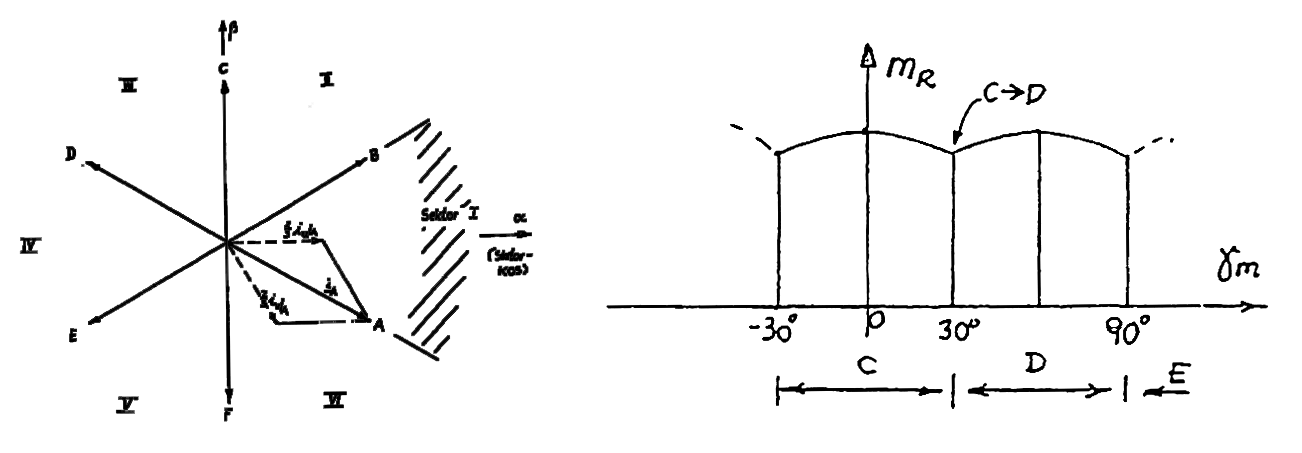
\includegraphics[scale=0.55]{2/BLDC.png}
    \caption{Diskrete Raumzeiger mit Sektoren im statorfesten KOS (links) und Momentenverlauf in Abhängigkeit der Rotorposition (rechts).}
    \label{fig:bldc_schema}
\end{figure}

%Finde ich ein wenig ungenau formuliert - bitte nicht köpfen, lg Thomas %Da der Stromraumzeiger für \SI{60}{\degree} Blöcke konstant bleibt, entsteht kein konstantes Drehmoment mehr, sondern ein cosinusförmiges laut folgender Gleichung
%\begin{equation*}
%    m_R(\tau) = - Im \left[ \underline{i}^*_s \underline{\Psi}_S\right] = - Im \left[ \underline{i}^*_s \big( \underline{\Psi}_M \big) \right] = \underline{\Psi}_M \cdot i_{s,d} = \underline{\Psi}_M  i_{s} \cdot sin(\gamma_m)
%\end{equation*}

\noindent Im Zuge eines erneuten Drehzahlsprunges wurden die Ströme in dieser Betriebsart gemessen. Diese sind als Stromortskurve in Abbildung \ref{fig:stromortskurve_bldc} dargestellt und zeigen die erwarteten diskreten Stromraumzeiger. Die abweichenden Stromraumzeiger, die mitten in den Sektoren zum Liegen kommen, sind auf ... ?? .. zurückzuführen.

\input{\currfiledir stromortskurve.tex}

\noindent Weiters ist der entsprechende Zeitverlauf der Messgrößen dieses Versuches in Abbildung \ref{fig:sprung_bldc} dargestellt. Eine Umrechnung der $\alpha, \beta$-Komponenten des Statorstromes in die entsprechenden Strangströme gemäß Gl. \ref{eq:umrechnung} liefert wiederum deren zeitlichen Verlauf in Abbildung \ref{fig:phasenstroeme_bldc} (wieder berechnet, nicht direkt gemessen). Es sind in beiden Diagrammen deutlich die diskreten Werte der Ströme und auch die für den BLDC-Betrieb charakteristische Schaltfolge zu erkennen, sowie die Tatsache, dass sich auch hier die Summe der Strangströme stets zu 0 addiert. Beim Drehzahlsprung ist beim Umkehrpunkt der Drehzahl auch der Lagewinkel $\gamma_m$ zufällig gleich 0, und man erkennt deswegen sehr gut, dass in diesem Fall (Fluss zeigt in die $\alpha$-Achse bzw. in Richtung des ersten Stranges) der Stromraumzeiger F ideal ist, da dieser dem Fluss zu diesem Zeitpunkt genau $90\degree$ voreilt (Linkslauf). Dieser Zeiger korrespondiert mit der negativen $\beta$-Achse, demzufolge ist auch der negative $i_{\beta}$ maximal und $i_{\alpha}$ gleich 0. Dies spiegelt sich ebenso in den Strangströmen wider, wo entsprechend $i_1$ gleich 0, $i_2$ negativ und $i_3$ positiv ist. Weiters ist anzumerken, dass es in den Strangströmen zu Stromeinbrüchen aufgrund der Schaltvorgänge kommt.\\
\noindent Abschließend wird ein weiterer Drehzahlsprung betrachtet, diesmal jedoch im d,q-KOS (vgl. Abbildung \ref{fig:umkehr_bldc_dq}). Zu sehen ist der qualitativ erwartete Verlauf des q-Stromes entsprechend des rechten Teils der Abb. \ref{fig:bldc_schema}, da der Fluss konstant und das wellige Moment damit proportional zur q-Stromkomponente ist. Dementsprechend ist im BLDC-Betrieb auch der d-Strom nur mehr dort 0, wo die Momentenausbeute ideal ist, und zeigt sonst ein Sägezahn-Verhalten: Bei jedem Umschaltvorgang wechselt die Projektion des diskreten Stromraumzeigers auf die d-Achse ihr Vorzeichen und nimmt betraglich ab, bis sie verschwindet, um dann mit dem Lagewinkel wieder bis zur nächsten Umschaltung betraglich zu steigen. Betrachtet man den maximalen Einbruch des Momentes und folglich der q-Stromkomponente im idealen Fall, so beträgt dieser $1-\cos(30\degree) \approx 0.13$. In der Messung tritt ein Einbruch von $\approx 0.25$ auf, also fast ein doppelt so großer Wert (?warum?).

\input{\currfiledir sprung_bldc.tex}
\input{\currfiledir phasenstroeme.tex}
\input{\currfiledir umkehr_bldc_dq.tex}

